\subsection{Representation and analysis stages}
SheetShrink removes redundant records from an XLSX ZIP package while preserving
workbook structure and cell coordinates. Before evaluating individual cells, it
reads styles, shared strings, relationships, merged regions and dependency sources.
A style index or empty value alone cannot establish redundancy.

Worksheet analysis reads decompressed bytes without creating an XML object for
each cell. A state machine distinguishes headers, columns, sheet data, merges and
the remaining XML. Tag and attribute readers track nesting and quotation marks,
preventing coordinate-like text in attribute values from being interpreted as cell
addresses. Partial markers are retained across buffer boundaries. Metadata is
retained when later decisions need it. Names, references and other interpreted
values may require decoding.

Memory use grows with worksheet size. SheetShrink retains sheet-data bytes,
analysis context and candidate metrics for later passes. Decompression, rewriting
and compression also contribute to peak memory. The supported format is
unprefixed Transitional SpreadsheetML. Unsupported namespaces, encodings and
ambiguous structures trigger preservation or exclusion~\cite{sheetshrinkcontract}.
Bounded package-header checks and declarations encountered during streaming
identify unsupported representations before opening in Excel.

Figure~\ref{fig:worksheet-states} shows how the worksheet parser dispatches column,
cell and merge readers. It retains partial state across buffer boundaries and
processes complete rows while retaining an unfinished row. Reconstruction requires
the worksheet end.
\begin{figure}[t]
\centering
\begin{tikzpicture}[x=1cm,y=1cm]
\node[state node] (seek) at (1,0) {Find root\\\texttt{worksheet}};
\node[state node] (scan) at (3.85,0) {Scan children};
\node[state final] (end) at (6.8,0) {End found};
\node[state node] (cols) at (1,-2.1) {Read columns\\\texttt{cols}};
\node[state work] (data) at (3.85,-2.1) {Read cells\\\texttt{sheetData}};
\node[state node] (merges) at (6.8,-2.1) {Read merges\\\texttt{mergeCells}};
\fill[stateSlate] (-.25,0) circle (1.5pt);
\draw[state edge] (-.25,0) -- (seek.west);
\draw[state edge] (seek) -- node[state label,above=8pt] {root found} (scan);
\draw[state edge] (scan) -- node[state label,above=8pt] {\texttt{</worksheet>}} (end);

\draw[state edge] (scan.south west) to[bend right=12]
  node[state label,above left,pos=.56] {open} (cols.north east);
\draw[state edge] (cols.north east) to[bend right=12]
  node[state label,below right,pos=.45] {close} (scan.south west);
\draw[state edge] (scan.south) to[out=-115,in=115]
  node[state label,left,pos=.5] {open} (data.north);
\draw[state edge] (data.north) to[out=65,in=-65]
  node[state label,right,pos=.5] {close} (scan.south);
\draw[state edge] (scan.south east) to[bend left=12]
  node[state label,above right,pos=.56] {open} (merges.north west);
\draw[state edge] (merges.north west) to[bend left=12]
  node[state label,below left,pos=.45] {close} (scan.south east);
\draw[state edge] (data.south west) to[out=-145,in=-35,looseness=2.3]
  node[state label,below] {emit complete rows} (data.south east);

\node[state note,text width=7.5cm,anchor=north west] at (0,-3.65)
  {Read boundaries retain state and unfinished input.};
\node[state error,text width=7.1cm,anchor=north west,minimum height=.6cm]
  at (.05,-4.15) {\textbf{Error return from unfinished states}\\
    Incomplete root/end, I/O failure or unsupported XML};
\end{tikzpicture}
\caption{The six worksheet-stream states. Child readers return to the same
worksheet dispatcher. Row-aligned progress retains a partial row across reads.
The lower box summarizes error outcomes. Reaching the end state permits
reconstruction, with workbook publication subject to its own completion checks.}
\label{fig:worksheet-states}
\end{figure}


\subsection{Parser correctness and regression controls}
The byte scanner must recognize XML structure and track parser state. It must
check element boundaries, quoted attributes, empty elements and incomplete input.
Established SAX and DOM parsers provide extensively tested syntax handling.
Memory-safe code can still misclassify content and produce an incorrect workbook.

Our development history supplies a concrete example. A Data.gov workbook used
\texttt{<v xml:space="preserve">} for visible string values. A scanner recognizing
only the literal \texttt{<v>} classified these cells as empty and removed a heading
and other strings. The correction recognizes valid element-name delimiters and
retains attributed value and inline-string elements. Negative controls reject
longer lookalike names such as \texttt{<value>}~\cite{attributedvaluefix}.
A separate defined-name regression ensures that a self-closing element cannot
consume the following paired element during replacement~\cite{definednamefix}.

The worksheet stream must reach its
closing state before output publication. An incomplete parse raises an error,
removes partial output and preserves any existing destination. Integration
fixtures exercise this failure after another worksheet has already been
processed~\cite{incompleteparsefix}. Streaming diagnostics additionally test
comments, CDATA, quotes, nesting limits and source offsets across every input
chunk size of their small fixtures.

At the time of writing, 31 correctness tests in the dedicated XML, namespace,
shared-string, range, defined-name and streaming-reader modules exercise parsing
and recognition behavior. A further 155 correctness tests in the cell, row and
tail suites cover preservation witnesses, inheritance masks and content
boundaries. Additional tests cover dependencies, styles, output construction and
execution behavior. Counts refer to test functions, with parameterized fixture
iterations counted once. The artifact records the source revision, test paths
and counting criteria.

\subsection{Effects and compact preservation witnesses}
A numeric value, formula or inline string is content. In particular, zero and a
shared-formula follower with no independent formula text remain content.
An empty cell is classified by its effective formatting in the cell, row and
column context. An explicit no-fill or borderless style can suppress a visible
inherited effect. It remains necessary whenever deletion would expose that
effect. Conversely, an explicit no-fill with nothing to clear can be redundant.
Style components and application flags are therefore interpreted together.

An empty cell's font can set automatic row height and shift later content.
SheetShrink keeps a required representative for repeated font records. Equivalent
fonts can share an identity despite different style indices. Column-font masks
and merged spans also constrain removal. A record elsewhere in the row may not
preserve a required local mask.
Figure~\ref{fig:font-witness-native} isolates the mechanism in a constructed
native Excel control. One witness preserves the observed height. Removing both
moves the next visible row.
\begin{figure}[t]
\centering
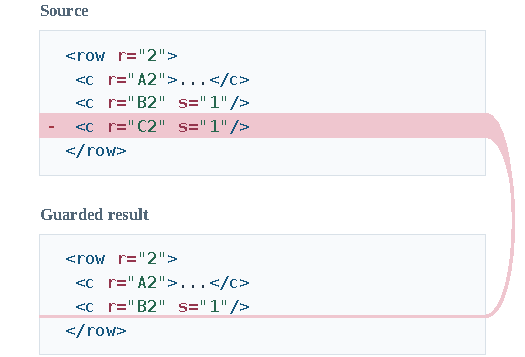
\includegraphics[width=\columnwidth]{figures/xml-methods/font-witness-code.pdf}
\par\smallskip
\begin{tabular}{@{}l@{\hspace{0.02\columnwidth}}c@{}}
Original & 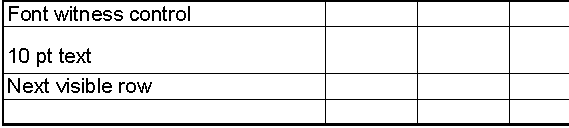
\includegraphics[width=0.70\columnwidth]{evidence/xml-methods/native-vector/font/source.pdf} \\
One witness & 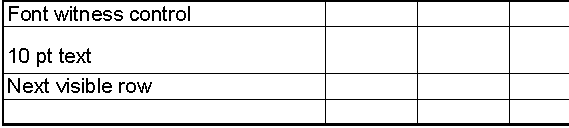
\includegraphics[width=0.70\columnwidth]{evidence/xml-methods/native-vector/font/one-witness.pdf} \\
No witness & 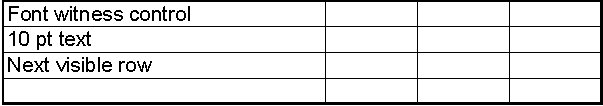
\includegraphics[width=0.70\columnwidth]{evidence/xml-methods/native-vector/font/no-witness.pdf}
\end{tabular}
\caption{Font-witness control. A2 uses Arial 10; empty B2 and C2 use Arial 18.
Retaining either blank preserves the rebuilt rendering. Removing both reduces
row 2 from 23.25 to 12.75 points and shifts the following row. XML is abbreviated;
images are native Excel print exports.}
\label{fig:font-witness-native}
\end{figure}


A fixed height eliminates this automatic-height effect, but an empty font-bearing
cell can still affect the text baseline in a row containing text. The cleaner
therefore distinguishes an empty fixed-height row from a fixed-height text row.
Protection metadata does not erase a required font contribution. Protection
formats inside the retained data extent also preserve interaction semantics,
while separately guarded exterior tails can be removed.

Other witnesses preserve relationships between coordinates. Center-across-selection
requires the contiguous blank span following the text cell. A borderless row can
mask column borders, and an empty height-bearing row can determine their vertical
extent. Column widths remain necessary when they support visible row borders.
A chart can inherit a number format from an empty first series cell. These
structures extend the preservation problem beyond the last nonempty value.
Figure~\ref{fig:fill-override-native} shows an Enron counterexample in which
Check Performance's smaller output exposes a different inherited fill. The
observation concerns the pictured rebuilt region.
\begin{figure*}[t]
\centering
\begin{tabular}{@{}c@{\hspace{0.015\textwidth}}c@{\hspace{0.015\textwidth}}c@{}}
Original & SheetShrink Default & Check Performance \\

\includegraphics[width=0.323\textwidth]{figures/xml-methods/fill-original-code.pdf} &

\includegraphics[width=0.323\textwidth]{figures/xml-methods/fill-sheetshrink-code.pdf} &

\includegraphics[width=0.323\textwidth]{figures/xml-methods/fill-check-performance-code.pdf} \\[2pt]
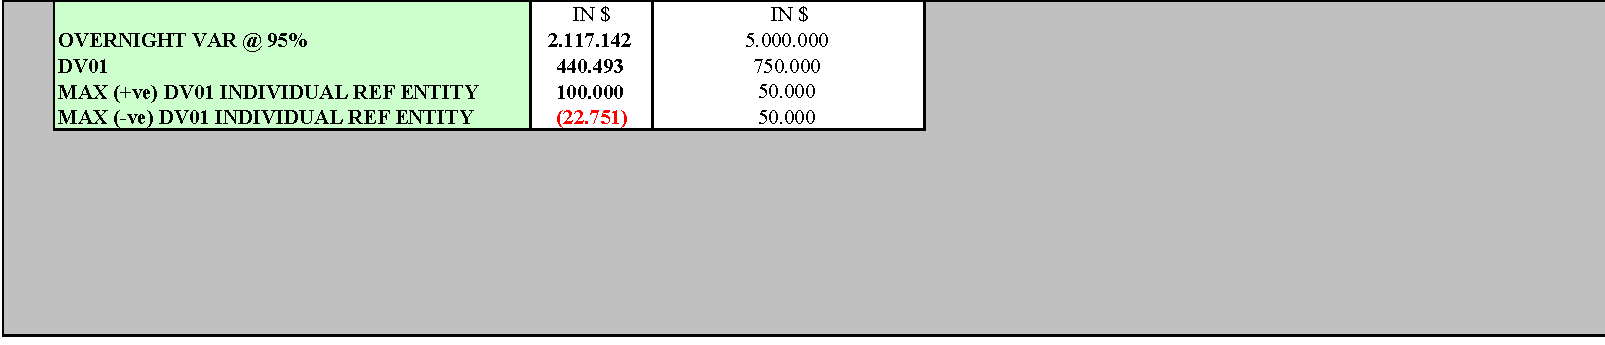
\includegraphics[width=0.323\textwidth]{evidence/xml-methods/native-vector/enron/Original.pdf} &
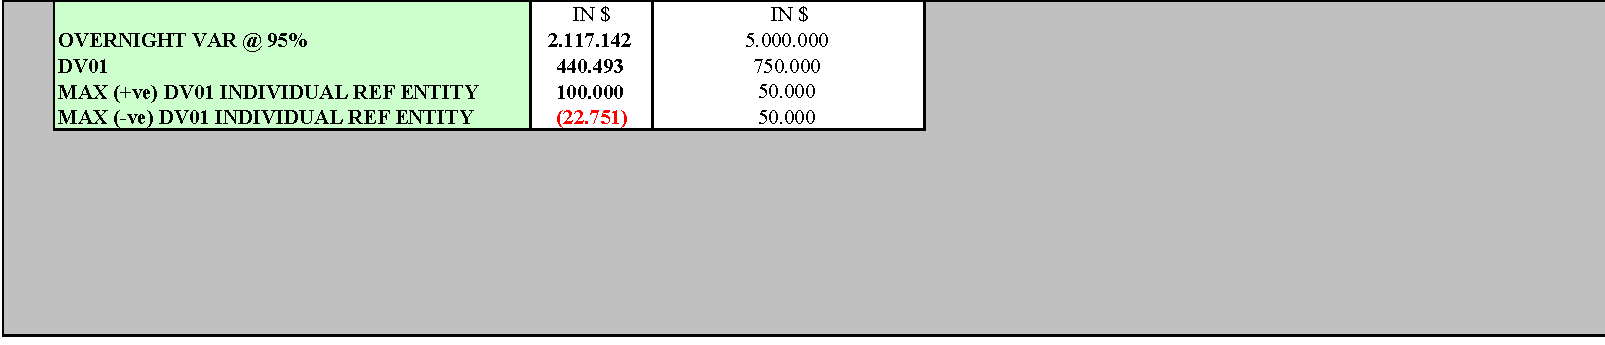
\includegraphics[width=0.323\textwidth]{evidence/xml-methods/native-vector/enron/Default.pdf} &
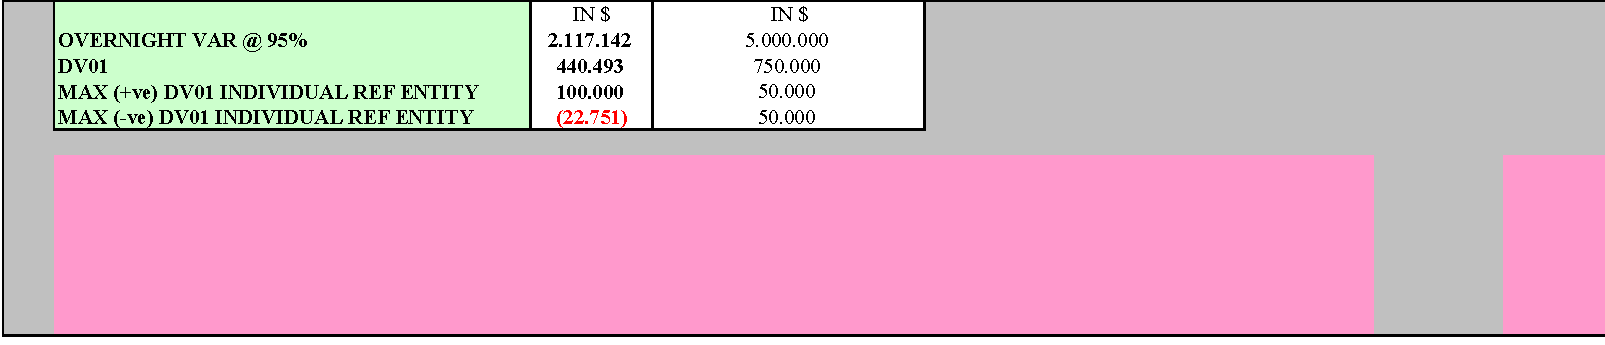
\includegraphics[width=0.323\textwidth]{evidence/xml-methods/native-vector/enron/Check-Performance.pdf}
\end{tabular}
\caption{An empty cell masks inherited formatting. In the Enron example, gray B31
overrides a pink column fill. SheetShrink preserves the mask; Check Performance
removes it and exposes pink. Native print exports match for Original and
SheetShrink after full rebuild within the displayed region. XML is abbreviated.}
\label{fig:fill-override-native}
\end{figure*}


\subsection{Guarded promotion and tail pruning}
SheetShrink can replace repeated cell styles with an existing cell style applied
to the row. The row must be visible, unprotected and have no row style. A stored
height and enabled \texttt{customHeight} flag are required. The \texttt{ht}
attribute alone permits automatic sizing. Content, merges, gaps and inherited
column formats must remain compatible with the row format.
Figure~\ref{fig:row-style-promotion} illustrates the full-width
case~\cite{rowpromotionfix}.
\begin{figure}[t]
\centering
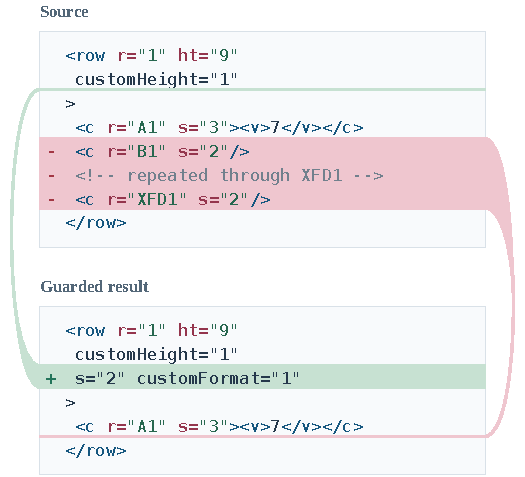
\includegraphics[width=\columnwidth]{figures/xml-methods/08-row-promotion.pdf}
\caption{Guarded dense-row promotion reuses an existing XF and keeps the value
cell. Red marks removed lines and green marks added lines. The illustration
omits the repeated middle cells. The full-width regression removes 16,383
empty cell records under the fixed-height and inheritance guards.}
\label{fig:row-style-promotion}
\end{figure}


The dominant empty-cell style occurs at least twice. Selection counts unsuitable
styles too, then applies eligibility checks. Otherwise an eligible minority
could incorrectly replace an unsuitable majority. Ties choose the smaller
existing style index. Dense promotion requires at least 1,024 occurrences.
A bounded-gap route admits at most 64 missing columns and restores required
original formats only under its inheritance checks. Sparse promotion requires
equivalent inheritance at every absent position and excludes merged sparse rows.
Uniform-fill promotion additionally checks content-cell fills. Unknown metadata
or style identities prevent promotion and retain the ordinary cleanup path.

Pruning removes formatting-only records beyond the last required content or
layout anchor. Font-only blanks beyond this boundary have no later content to
shift. Fills, borders, conditional formatting and drawings can extend the boundary.
A white row fill is redundant only if compatible column fills cover every column
through XFD. Compatible column ranges can be merged while preserving local
overrides and geometry needed for borders.

\subsection{Hidden content and the Wanderungen case}
\label{sec:wanderungen}
SheetShrink uses a conservative heuristic to remove certain hidden numeric tails.
A candidate must contain at least 4,096 identical integers and extend to XFD.
This restriction targets large repeated tails such as those in Wanderungen.
Candidates must also pass cell-level layout and dependency checks.
Gaps, formulas, text, differing values and unsupported numeric forms reject the
band. Source cells contribute before style cleanup. The common zero path compares
value bytes directly, while one admitted row span replaces per-cell entries in
the later reference map. Temporary row-local candidates still exist.

The motivating migration workbook contains 21 such zero tails in
\texttt{Tabelle 3.4}: rows 11--30 and 32, from L through XFD. Each contains
16,373 zeros, totaling 343,833. Source ZIP inspection confirms these counts and
retains the source hash. The historical cleanup investigation records 376,573
removed zeros across two worksheets, alongside 243 preserved nonzero values and
a retained short 237-zero tail~\cite{hiddentailcase}. These are content removals under an
explicit structural policy. A deliberate constant full-width matrix can meet
the same heuristic, so repetition alone does not establish user intent.

\subsection{Workbook dependencies and deferred rewriting}
SheetShrink postpones reference-sensitive deletions until it has checked supported
formulas, names, charts, objects and pivot dependencies across the workbook.
This includes references from later worksheets. Workbook relationships and sheet
scope identify reference targets. Shared-formula followers shift relative axes
and preserve absolute axes. The implementation protects enclosing referenced
ranges without enumerating each shared-formula follower's references. Dynamic
or unresolved references and unsupported expressions block deletion~\cite{sheetshrinkcurrentcontract}.

A known reference intersecting an admitted hidden span protects the entire span.
Only admitted candidates reach rewriting. Removing a payload need not remove its
format if that format still masks an inherited effect. After deferred changes,
affected rows lose their stale tail anchors and pass through cleanup again.
Otherwise records retained solely because of the removed anchor would survive
incorrectly. Whitespace removal is disabled in Default because whitespace can
control text overflow and row layout.

Package metadata has separate predicates. Calculation-chain cleanup resolves
removed cells by sheet identity and preserves unresolved mappings. The cleaner
does not evaluate formulas or manufacture replacement caches. Built-in alias
cleanup currently matches name and local scope without proving equality of the
two formula bodies.

\subsection{Parallel work and output ownership}
Figures~\ref{fig:hierarchical-scheduling} and~\ref{fig:schedule-execution}
show the task hierarchy and a schematic execution across threads. Worksheet identity remains shared across
its chunks, while ordered assembly separates execution order from output order.
\begin{figure}[t]
\centering
\begin{tikzpicture}[x=1cm,y=1cm,
  task/.style={rounded corners=2pt,draw=stateSlate!45,fill=white,
    minimum height=.48cm,inner sep=3pt,font=\scriptsize,align=center},
  edge/.style={-{Stealth[length=3pt]},draw=stateSlate!75,line width=.6pt},
  small/.style={font=\scriptsize,text=stateSlate,align=center}]
\definecolor{scheduleAmber}{HTML}{AD762B}
\path[use as bounding box] (-.45,.05) rectangle (5.55,-4.9);

\node[task,text width=1.45cm] (w1) at (1,-.45) {Workbook 1};
\node[task,text width=1.45cm] (w2) at (4,-.45) {Workbook 2};
\node[task,draw=stateBlue,fill=stateBlue!9] (a) at (.45,-1.55) {Sheet A};
\node[task,draw=stateTeal,fill=stateTeal!10] (b) at (2.1,-1.55) {Sheet B};
\node[task,draw=scheduleAmber,fill=scheduleAmber!10] (c) at (4.55,-1.55) {Sheet C};
\draw[edge] (w1) -- (a);
\draw[edge] (w1) -- (b);
\draw[edge] (w2) -- (c);
\foreach \id/\xx in {1/.7,2/2.1,3/3.5} {
  \node[task,draw=stateTeal,fill=stateTeal!10,minimum width=1cm]
    (chunk\id) at (\xx,-2.7) {B\,\id};
  \draw[edge] (b) -- (chunk\id);
}
\node[task,text width=2.45cm] (join) at (2.1,-3.8) {Assemble B\,1, B\,2, B\,3};
\foreach \id in {1,2,3} {\draw[edge] (chunk\id) -- (join);}
\node[small,anchor=north,text width=5.2cm] at (2.3,-4.25)
  {Complete rows stay together.\\Chunk results retain source order.};

\end{tikzpicture}
\caption{Task hierarchy. Workbook admission bounds active inputs; sheets and
row-aligned chunks share the Rayon pool. B\,1--B\,3 belong to one worksheet
and are assembled in source order. Colors match Figure~\ref{fig:schedule-execution}.}
\label{fig:hierarchical-scheduling}
\end{figure}

\begin{figure}[t]
\centering
\begin{tikzpicture}[x=1cm,y=1cm,
  small/.style={font=\scriptsize,text=stateSlate,align=center},
  edge/.style={-{Stealth[length=3pt]},draw=stateSlate!75,line width=.6pt}]
\definecolor{scheduleAmber}{HTML}{AD762B}
\path[use as bounding box] (0,.1) rectangle (8.3,-3.35);
\foreach \yy/\name in {-.45/1,-1.25/2,-2.05/3} {
  \draw[stateSlate!14,line width=.4pt] (1.2,\yy-.3) -- (8.1,\yy-.3);
  \node[small,anchor=east] at (1.1,\yy) {Thread \name};
}
\foreach \xx in {1.3,2.6,3.9,5.2,6.5,7.8} {
  \draw[stateSlate!10,line width=.35pt] (\xx,-.05) -- (\xx,-2.45);
}
\filldraw[fill=stateTeal!12,draw=stateTeal!65,rounded corners=1.5pt]
  (1.3,-.69) rectangle (2.15,-.21);
\node[small] at (1.725,-.45) {B init};
\filldraw[fill=stateTeal!22,draw=stateTeal,rounded corners=1.5pt]
  (2.25,-.69) rectangle (5.1,-.21);
\node[small] at (3.675,-.45) {B\,1};
\filldraw[fill=stateBlue!17,draw=stateBlue,rounded corners=1.5pt]
  (1.3,-1.49) rectangle (2.6,-1.01);
\node[small] at (1.95,-1.25) {A};
\filldraw[fill=stateTeal!38,draw=stateTeal,line width=.9pt,rounded corners=1.5pt]
  (2.7,-1.49) rectangle (5.8,-1.01);
\node[small] at (4.25,-1.25) {B\,2};
\filldraw[fill=scheduleAmber!19,draw=scheduleAmber,rounded corners=1.5pt]
  (1.3,-2.29) rectangle (2.35,-1.81);
\node[small] at (1.825,-2.05) {C};
\filldraw[fill=stateTeal!22,draw=stateTeal,rounded corners=1.5pt]
  (2.45,-2.29) rectangle (4.7,-1.81);
\node[small] at (3.575,-2.05) {B\,3};
\draw[stateTeal!65,dashed,line width=.6pt] (5.8,-2.45) -- (5.8,-.05);
\filldraw[fill=stateTeal!12,draw=stateTeal!65,rounded corners=1.5pt]
  (5.9,-.69) rectangle (7.5,-.21);
\node[small] at (6.7,-.45) {B finalize};
\node[small,anchor=north] at (5.8,-2.5) {All B chunks joined};
\draw[edge] (1.3,-3.15) -- (8.1,-3.15);
\node[small,fill=white,inner sep=2pt] at (4.7,-3.15) {Relative time};
\end{tikzpicture}
\caption{One possible execution of Figure~\ref{fig:hierarchical-scheduling}.
Chunks from one sheet can run on different threads before ordered assembly.
Bar lengths are schematic; individual steal events are not recorded.}
\label{fig:schedule-execution}
\end{figure}

Workbook, worksheet and row-chunk work share the cleanup execution budget.
A permit limits active workbooks and remains held through output finalization.
Workers can process other workbooks while one long worksheet remains active.
Large worksheets expose row-aligned chunks to Rayon, allowing idle workers to
help without splitting a row's font, promotion or tail decisions.
The chunk planner estimates byte-sized work, then adjusts boundaries to complete
rows. Small ranges use the serial path. Each chunk receives isolated metrics,
and results are assembled in source order.

Ready chunks participate in admission decisions for new worksheets. A smaller
sheet can yield admission while larger chunk work is pending. Batches retain only a bounded number of chunk results while the
assembled output grows. Workbook contexts, the output buffer and deferred
candidates remain additional memory consumers. Thread count, active-workbook
count and writer count are separate experimental parameters.

Workers compress changed worksheet members in parallel. One writer updates each
workbook's ZIP archive and publishes the completed temporary file after successful
processing. Unchanged members can reuse their compressed bytes. If every member
is unchanged, SheetShrink copies the original file byte for byte. A fast identity
check uses CRC32 and uncompressed size.

The method retains existing style and shared-string indices rather than globally
renumbering their tables. This avoids unrelated rewrites and permits copy-through
of unaffected members. It also leaves reductions requiring native save or global
table compaction outside the cleanup subject.
